\chapter{Graphs}

\begin{figure}[H]
    \tikzset{ every node/.style={draw, circle, minimum size=2em} }
    \centering
    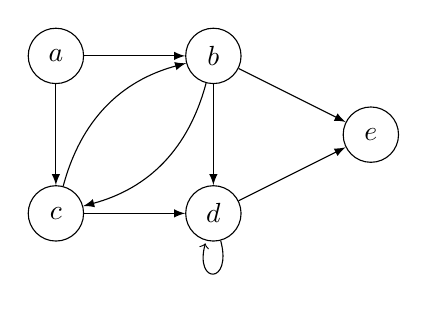
\begin{tikzpicture}[every edge/.style={draw, -latex}] 
        \node (a) at (0,0) {$a$};
        \node (b) at (2,0) {$b$};
        \node (c) at (0,-2) {$c$};
        \node (d) at (2,-2) {$d$};
        \node (e) at (4,-1) {$e$};

        \path (a) edge (b)
              (a) edge (c)
              (b) edge[bend left] (c)
              (b) edge (d)
              (b) edge (e)
              (c) edge[bend left] (b)
              (c) edge (d)
              (d) edge[loop below] (d)
              (d) edge (e);
    \end{tikzpicture}
    \hfil
    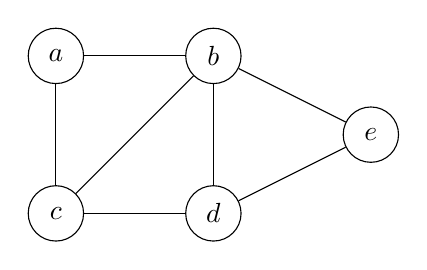
\begin{tikzpicture}
        \node (a) at (0,0) {$a$};
        \node (b) at (2,0) {$b$};
        \node (c) at (0,-2) {$c$};
        \node (d) at (2,-2) {$d$};
        \node (e) at (4,-1) {$e$};

        \path (a) edge (b)
              (a) edge (c)
              (b) edge (c)
              (b) edge (d)
              (b) edge (e)
              (c) edge (d)
              (d) edge (e);
    \end{tikzpicture}
\end{figure}

\section{Graphs}

\subsection{Graphs}

Define a graph $G = \{ V, E \}$

\subsubsection{Representations}

\listu {
    \item Adjacency matrix
    
    \begin{center} \begin{tabular}{c | c c c c c}
            & $a$ & $b$ & $c$ & $d$ & $e$ \\ \hline
        $a$ & 0   & 1   & 1   & 0   & 0   \\
        $b$ & 1   & 0   & 1   & 1   & 1   \\
        $c$ & 1   & 1   & 0   & 1   & 0   \\
        $d$ & 0   & 1   & 1   & 0   & 1   \\
        $e$ & 0   & 1   & 0   & 1   & 0
    \end{tabular} \end{center}

    Complexity: let $n = |V|$ and $m = |E|$
    \listu {
        \item Space: $O(n^2)$
        \item Edge query: $\Theta(1)$ time
    }

    \item Adjacency list
    
    % TODO: add figure

    Complexity: let $n = |V|$ and $m = |E|$
    \listu {
        \item Space: $\Theta(n + m)$
        \item Edge query: $\Theta(n)$ in worst-case time
    }
}

\subsection{Breadth-First Search}

In breadth first search, we start at a source $s \in V$, and explore every vertex reachable from $a$, using only edges. 

\begin{figure}[H]
    \centering
    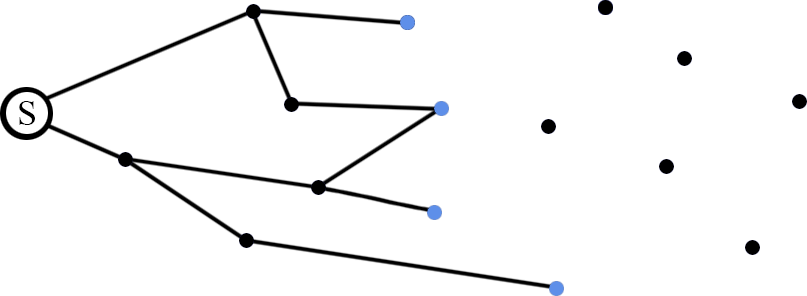
\includegraphics[width=0.5\linewidth]{images/BFS.png}
\end{figure}

We assign each vertex $v \in V$ a color, which can be one of the following:
\listu {
    \item White: $v$ has not been discovered
    \item Gray: $v$ has been discovered, but not explored
    \item Black: $v$ has been discovered and explored
}

Define $\pi[v]$ to be the predecessor of $v$ in the breadth-first search tree.

Define $d[v]$ to be the distance from $s$ to $v$ in the breadth-first search tree.

We use a queue to keep track of the vertices that we have discovered, but not yet explored.

\clearpage

\begin{algorithm}[H] \begin{algorithmic}[1]
    \Procedure{BFS}{$G$, $s$}
        \State \cmt{Initialize tracking info for all vertices}
        \For {$v \in G.V$}
            \State colour[$v$] = white
            \State $\pi[v] \gets \text{NIL}$
            \State $d[v] \gets \infty$
        \EndFor

        \State \cmt{Initialize empty queue and source vertex tracking info}
        \State $Q \gets \textsc{Make-queue}()$
        \State $\text{colour}[s] \gets \text{gray}$
        \State $\pi[s] \gets \text{NIL}$
        \State $d[s] \gets 0$
        \State \textsc{Enqueue}($Q$, $s$)

        \State \cmt{Main loop. Loop Invariant: $Q$ contains all (and only) gery vertices}
        \While {$Q \neq \textsc{Empty-queue}$}
            \State $u \gets \textsc{Dequeue}()$
            \For {$v \in G.Adj[u]$}
                \If {$\text{colour}[v] \gets \text{white}$}
                    \State $\text{colour}[v] \gets \text{gray}$
                    \State $\pi[v] \gets u$
                    \State $d[v] \gets d[u] + 1$
                    \State \textsc{Enqueue}($Q$, $v$)
                \EndIf
            \EndFor
            \State $\text{colour}[u] = \text{black}$
        \EndWhile
    \EndProcedure
\end{algorithmic} \end{algorithm}

In breath first search, \listu {
    \item Each vertex is enqueued at most once
    \item Each vertex is dequeued at most once
    \item Each adjacent list is examined at most once
    \item The time complexity is $\Theta(n + m)$
}

\subsubsection*{BFS Finds Shortest Paths}

Define $\delta(s, v)$ to be the length of the shortest path from vertex $s$ to vertex $v$ (i.e. the smallest number of edges in any path from $s$ to $v$). If there is no path from $s$ to $v$, then $\delta(s, v) = \infty$. Note that this definition will change when we consider \bred{weighted} graphs.

\theorem { 
    \label{thm:bfs-shortest-path} 
    Let $G = \{ V, E \}$ be a graph, and let $s \in V$. Then, after \textsc{BFS}($G$, $s$), $\forall v \in V$, $\delta(s, v) = d[v]$
}

To prove this theorem, we will need to prove the following lemmas first.

\lemma {
    \label{lem:bfs-shortest-path-1}
    $\forall (u, v) \in E$, $\delta(s, v) \leq \delta(s, u) + 1$
}

\begin{proof}
    (idea)

    If $\delta(s, u) = \infty$, then the claim holds trivially. 

    If $\delta(s, u) \neq \infty$, then $u$ is reachable from $s$.

    Thus, $v$ is also reachable from $s$.

    Thus, the shortest path from $s$ to $v$ is no longer than the shortest path from $s$ to $u$, plus the edge $(u, v)$.

    Hence, $\delta(s, v) \leq \delta(s, u) + 1$.
\end{proof}

\lemma {
    \label{lem:bfs-shortest-path-2}
    At ant point during BFS, $\forall v \in V$, $d[v] \geq \delta(s, v)$
}

\begin{proof}
    (idea)

    Use induction on the number of \textsc{Enqueue} operations.

    Immediately after we do the first \textsc{Enqueue} operation, $d[s] = 0$, and $\delta(s, s) = 0$.

    We also have $d[v] = \infty$, and $\delta(s, v) = \infty$ for all $v \in V - \{ s \}$.

    Now, consider some vertex $v$ that is first discovered while visiting a vertex $u$.

    By the IH, we have $d[u] \geq \delta(s, u)$.

    Hence, $d[v] = d[u] + 1 \geq \delta(s, u) + 1$ by Lemma 4.2.1. %TODO: use \ref

    Then $v$ is painted grey and $d[v]$ is not changed for the rest of the algorithm.
\end{proof}

\lemma {
    \label{lem:bfs-shortest-path-3}
    If $Q = \left< v_1, \dots, v_r \right>$, then $d[v_i] \leq d[v_{i+1}]$ for all $i \in \{ 1, \dots, r-1 \}$ and $d[v_r] \leq d[v_1] + 1$
}

\begin{proof}
    (sketch)

    Use induction on the number of \textsc{Dequeue} / \textsc{Enqueue} operations.

    When $Q = \left< s \right>$, the claim holds trivially.

    To prove the inductive step, we need to show that the lemma hold after applying \textsc{Dequeue} / \textsc{Enqueue} to $Q = \left< v_1, \dots, v_3 \right>$.

    \begin{itemize}
        \item Case 1
        
        If we perform a \textsc{Dequeue} operation, then $Q = \left< v_2, \dots, v_3 \right>$ afterwards.

        By the IH, $d[v_r] \leq d[v_1] + 1$ and $d[v_1] \le d[v_2]$.

        Hence, $d[v_r] \leq d[v_2] + 1$.

        All other inequalities are unaffected. 

        \item Case 2 
        
        If we perform a \textsc{Enqueue} operation, then $Q = \left< v_1, \dots, v_{r+1} \right>$ afterwards.

        We discover $v_{r+1}$ while visiting some vertex $u$, so $d[v_{r+1}] = d[u] + 1$.

        Vertex $u$ must have been the previous vertex dequeued from the queue. 

        Hence, either $v_1$ was discovered while visiting $u$, in which case $[v_1] = d[u] + 1$, or $Q$ was equal to $\left< u_2, v_1, \dots \right>$ at some prior point, in which case $d[u] \leq d[v_1]$ by IH.

        Hence, $d[v_{r+1}] = d[u] + 1 \leq d[v_1] + 1$.

        Otherwise, $d[v_r] \leq d[u] + 1 = d[v_{r+1}]$ by the IH. 
    \end{itemize}
\end{proof}

Now, we can prove the theorem.

\begin{proof}
    To derive a contradiction, suppose $d[v] \neq \delta(s, v)$ for some vertex $v \in V$.

    Suppose $v$ is a vertex with minimal $\delta(s, v)$ for which this is satisfied.

    By Lemma 4.1.2, we have $d[v] > \delta(s, v)$.

    % TODO: add a figure

    Because we chose $v$ with minimal $\delta(s, v)$, we have $d[u] = \delta(s, u)$.

    Hence, $d[v] > \delta(s, v) = \delta(s, u) + 1 = d[u] + 1$.

    Consider the colour of $v$ when we first dequeue $u$ from $Q$.

    \begin{itemize}
        \item If $v$ is painted \textbf{white}, then we set $d[v] = d[u] + 1$, which is a contradiction.
        \item If $v$ is painted \textbf{black}, then $v$ was in the queue before $u$. By Lemma 4.1.3, we have $d[v] \le d[u]$, which is a contradiction.
        \item If $v$ is painted \textbf{grey}, then $v$ was discovered while visiting some vertex $w$ that was dequeued earlier than $u$. Hence, $d [v] = d[w] + 1$, and by Lemma 4.1.3 we have $d[w] \le d[u]$. So $d[v] \le d[u] + 1$, which is a contradiction.
    \end{itemize}
\end{proof}

\subsubsection{Time complexity of BFS}

\listu {
    \item Initialization (painting vertices white, setting entries of $d$ to $\infty$ and entries of $\pi$ to NIL) takes $\Theta(|V|)$ time. 
    \item After initialization, we never paint a vertex white.
    \item Thus, each vertex is enqueued/dequeued at most once. 
    \item Hence, we spend $\mathcal{O}(|V|)$ time doing queue operations. 
    \item Every time we dequeue a vertex, we scan its out-neighbourhood to discover its neighbours:
    \listu {
        \item With an \textbf{adjacency list}, we consider each edge at most once (or at most twice in an undirected graph), so in total we need at most $\mathcal{O}(|E|)$ time to consider all of the edges.
        \item With an adjacency matrix, we scan each row of the matrix at most once, so in total we need at most $\mathcal{O}(|V|^2)$ time to consider all of the edges.
    }
}

\begin{minipage}[t]{0.45\linewidth} \begin{center}
    Using adjacency list: $\mathcal{O}(|V| + |E|)$
\end{center} \end{minipage}
\begin{minipage}[t]{0.45\linewidth} \begin{center}
    Using adjacency matrix: $\mathcal{O}(|V|^2)$
\end{center} \end{minipage}

\subsection{Depth-First Search}

\listu {
    \item In DFS, we walk through the graph as far as possible until we hit a dead end -- when this happens, we backtrack to an undiscovered vertex. 
    \item Similar to BFS, we paint vertices as we go: 
    \listu {
        \item Painted white: undiscovered
        \item Painted grey: discovered but not yet visited 
        \item Painted black: visited
    }
    \item Instead of storing distances/depths, we store timestamps: 
    \item \listu {
        \item $\textit{disc}[v] = \null$time at which $v$ is first discovered
        \item $\textit{vis}[v] = \null$time at which we finish visiting $v$
    }
}

\listu {
    \item One approach is to simply replace the \itblue{queue} from the BFS algorithm with a \itblue{stack}. This gives us an \bred{iterative} DFS algorithm. 
    \item However, it is more natural to write DFS as a recursive algorithm.
}

\begin{minipage}[t]{0.45\linewidth} \begin{algorithm}[H] \begin{algorithmic}[1]
    \Procedure{DFS}{G}
        \State \cmt{Initialization}
        \For {each $v \in G.V$}
            \State $d[v] \gets f[v] \gets \infty$
            \State $\pi[v] \gets \text{NIL}$
        \EndFor
        \State $\text{time} \gets 0$  \cmt{global}
        \State \cmt{Main loop}
        \For {each $v \in G.V$}
            \If {$d[v] = \infty$} 
                \State \cmt{colour[$v$] = white}
                \State \Call{DFS-Visit}{$G$, $v$}
            \EndIf
        \EndFor
    \EndProcedure
\end{algorithmic} \end{algorithm} \end{minipage}
\hfill
\begin{minipage}[t]{0.45\linewidth} \begin{algorithm}[H] \begin{algorithmic}[1]
    \Procedure{DFS-Visit}{$G$, $v$}
        \State \cmt{Discovered (colour[v] = grey)}
        \State $d[v] \gets \text{time} \gets \text{time} + 1$
        \State \cmt{Do something with $v$, if desired}
        \State \cmt{Explore $v$'s adjacency list}
        \For {each $u \in G.adj[v]$}
            \If {$d[u] = \infty$} 
                \State \cmt{colour[$u$] = white}
                \State $\pi[u] = v$
                \State \Call{DFS-Visit}{$G$, $u$}
            \EndIf
        \EndFor
        \State \cmt{Finished (colour[$v$] = black)}
        \State $f[v] \gets \text{time} \gets \text{time} + 1$
    \EndProcedure
\end{algorithmic} \end{algorithm} \end{minipage}

\subsubsection{DFS Forests}

We classify each edge $(u, v)$ based on the colour of $v$ when we consider this edge:

\listu {
    \item \term{Tree edges} are the edges $u$, $v \in E$ that form the DFS forest stored by $\pi$ 
    
    The vertex $v$ is painted \bred{white} when $(u, v)$ is considered 

    \item \term{Back edges}\index{DFS Tree!Back Edge} are the edges $(u, v) \in E$ such that $v$ is an ancestor of $u$ in the DFS forest 
    
    The vertex $v$ is painted \bred{grey} when $(u, v)$ is considered

    \item \term{Forward edges}\index{DFS Tree!Forward Edge} are the edges $(u, v) \in E$ such that $v$ is a descendant of $u$ in the DFS forest 
    
    The vertex $v$ is painted \bred{black} when $(u, v)$ is considered

    \item \term{Cross edges}\index{DFS Tree!Cross Edge} are all other edges $(u, v) \in E$ that are not part of the DFS forest (i.e. $v$ is neither an ancestor nor a descendant of $u$)

    The vertex $v$ is painted \bred{black} when $(u, v)$ is considered
}

\begin{figure}[H]
    \centering
    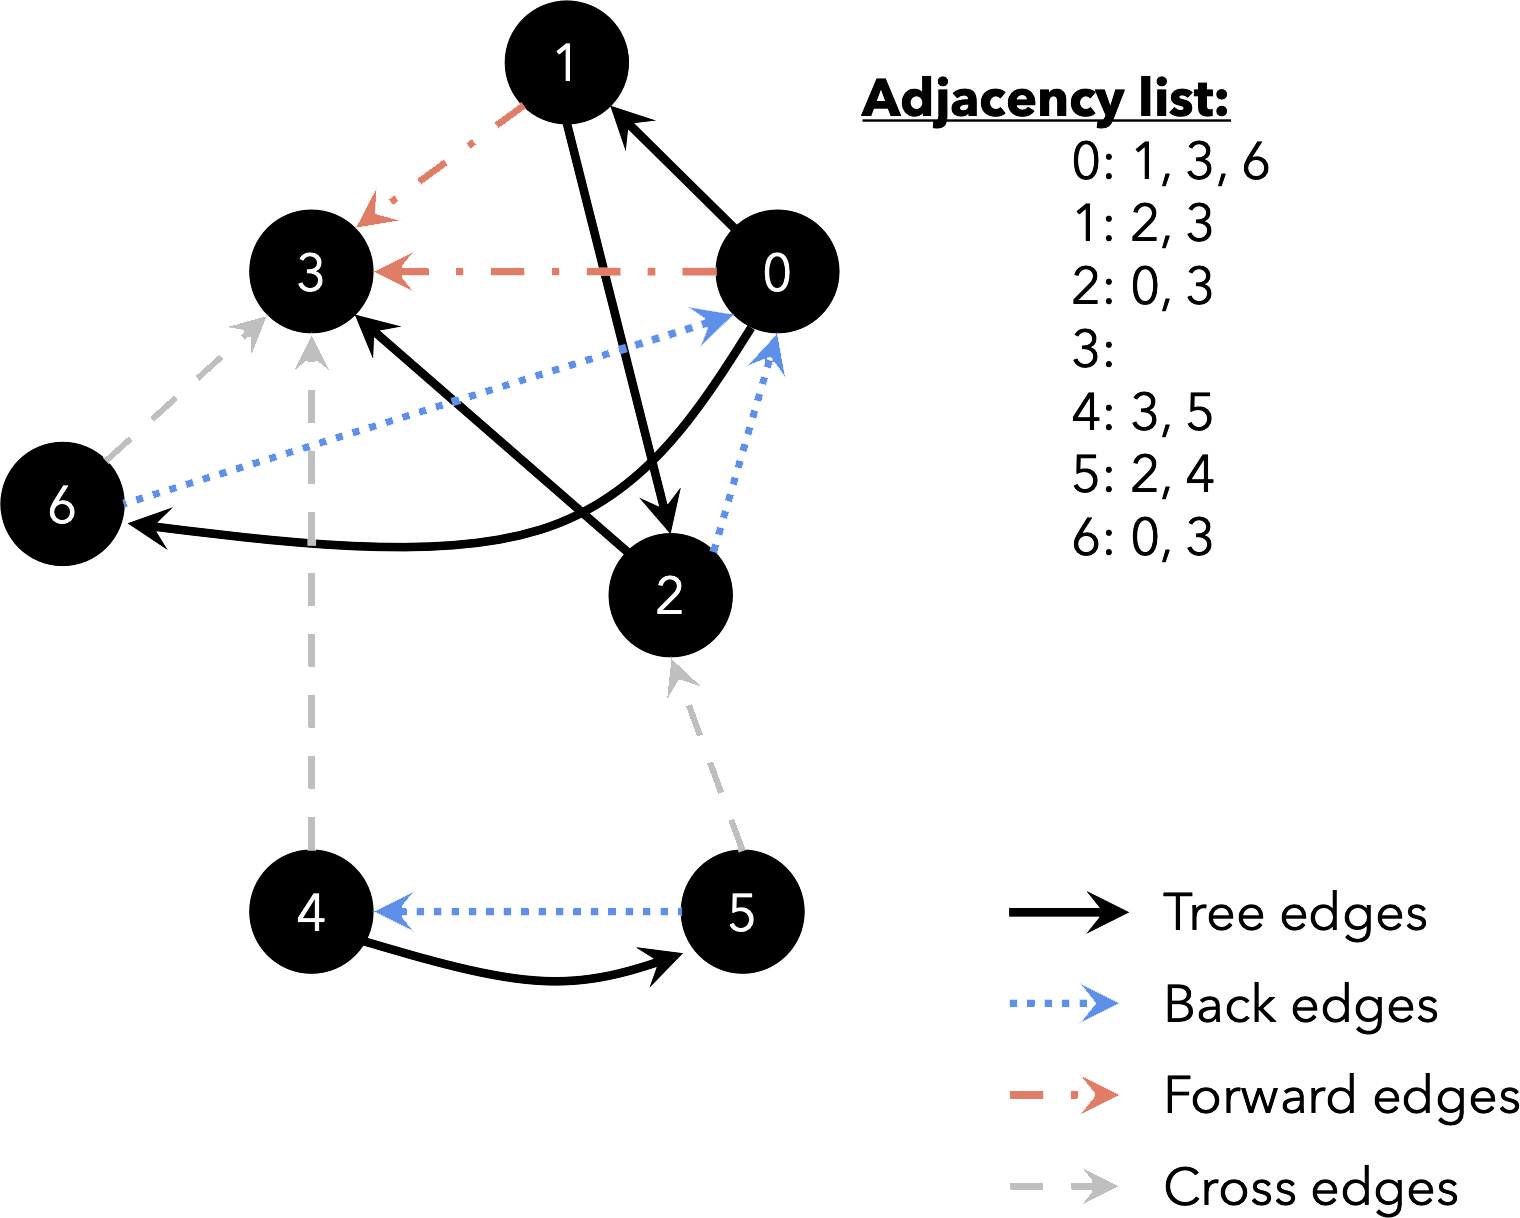
\includegraphics[width=0.5\linewidth]{images/DFS-Tree_Edges.png}
\end{figure}

Note that for undirected graphs, there are NO forward edges and NO cross edges.

\subsubsection{Time Complexity}

The run-time of DFS is similar to BFS.

\begin{minipage}[t]{0.45\linewidth} \begin{center}
    Using adjacency list: $\mathcal{O}(|V| + |E|)$
\end{center} \end{minipage}
\begin{minipage}[t]{0.45\linewidth} \begin{center}
    Using adjacency matrix: $\mathcal{O}(|V|^2)$
\end{center} \end{minipage}

\subsubsection{Parenthesis theorem}\index{Parenthesis Theorem}

\theorem {
    After performing \textsc{DFS}$(G = (V, E))$, for any two vertices $u$, $v \in V$, exactly one of the following statements holds:
    \listo {
        \item The intervals $\left[ \textit{disc}[u], \textit{vis}[u] \right]$ and $\left[ \textit{disc}[v], \textit{vis}[v] \right]$ are disjoint, and neither $u$ nor $v$ is a descendant of the other in the DFS forest.
        \item The interval $\left[ \textit{disc}[u] , \textit{vis}[u] \right]$ is contained entirely in the interval $\left[ \textit{disc}[v], \textit{vis}[v] \right]$, and $u$ is a descendant of $v$ in the DFS forest.
        \item The interval $\left[ \textit{disc}[v], \textit{vis}[v] \right]$ is contained entirely in the interval $\left[ \textit{disc}[u], \textit{vis}[u] \right]$, and $v$ is a descendant of $u$ in the DFS forest.
    }
}

\begin{proof}
    (sketch)

    Suppose that $\textit{disc}[u] < \textit{disc}[v]$.

    \listu {
        \item Case 1: $\textit{disc}[v] < \textit{vis}[u]$

        \begin{center} 
            \includegraphics*[width=0.2\linewidth]{images/Parenthesis-Thm-Grey-u.png}

            $v$ is first discovered while $u$ is painted grey.  
        \end{center}

        So $v$ is a descendant of $u$.

        We don't backtrack to $u$ until we have finished visiting $v$.

        Therefore, we paint $v$ black and set $\textit{vis}[v]$ before backtracking to $u$. Hence, $\textit{vis}[v] < \textit{vis}[u]$.

        \item Case 2: $\textit{vis}[u] < \textit{disc}[v]$

        \begin{center} \includegraphics*[width=0.2\linewidth]{images/Parenthesis-Thm-Black-u.png}

            $v$ is first discovered while $u$ is painted black.  
        \end{center}

        So $v$ is not a descendant of $u$.

       Since $\textit{disc}[u] < \textit{dics}[v]$, $u$ is not a descendant of $v$.

       Since $\textit{disc}[u] < \textit{vis}[u]$ and $\textit{disc}[v] < \textit{vis}[v]$, we have $\textit{disc}[u] < \textit{vis}[u] < \textit{disc}[v] < \textit{vis}[v]$.
    }

    When $\textit{disc}[v] < \textit{disc}[u]$, proof is symmetric.
\end{proof}

\subsection{Strongly connected}

Recall that an undirected graph is connected if and only if there is a path of edges between any pair of vertices in $V$. What about directed graphs? A directed graph $G = (V, E)$ is strongly connected if and only if, for all $u$, $v \in V$, there is a path of edges from $u$ to $v$ in $G$. 

\begin{figure}[H]
    \centering
    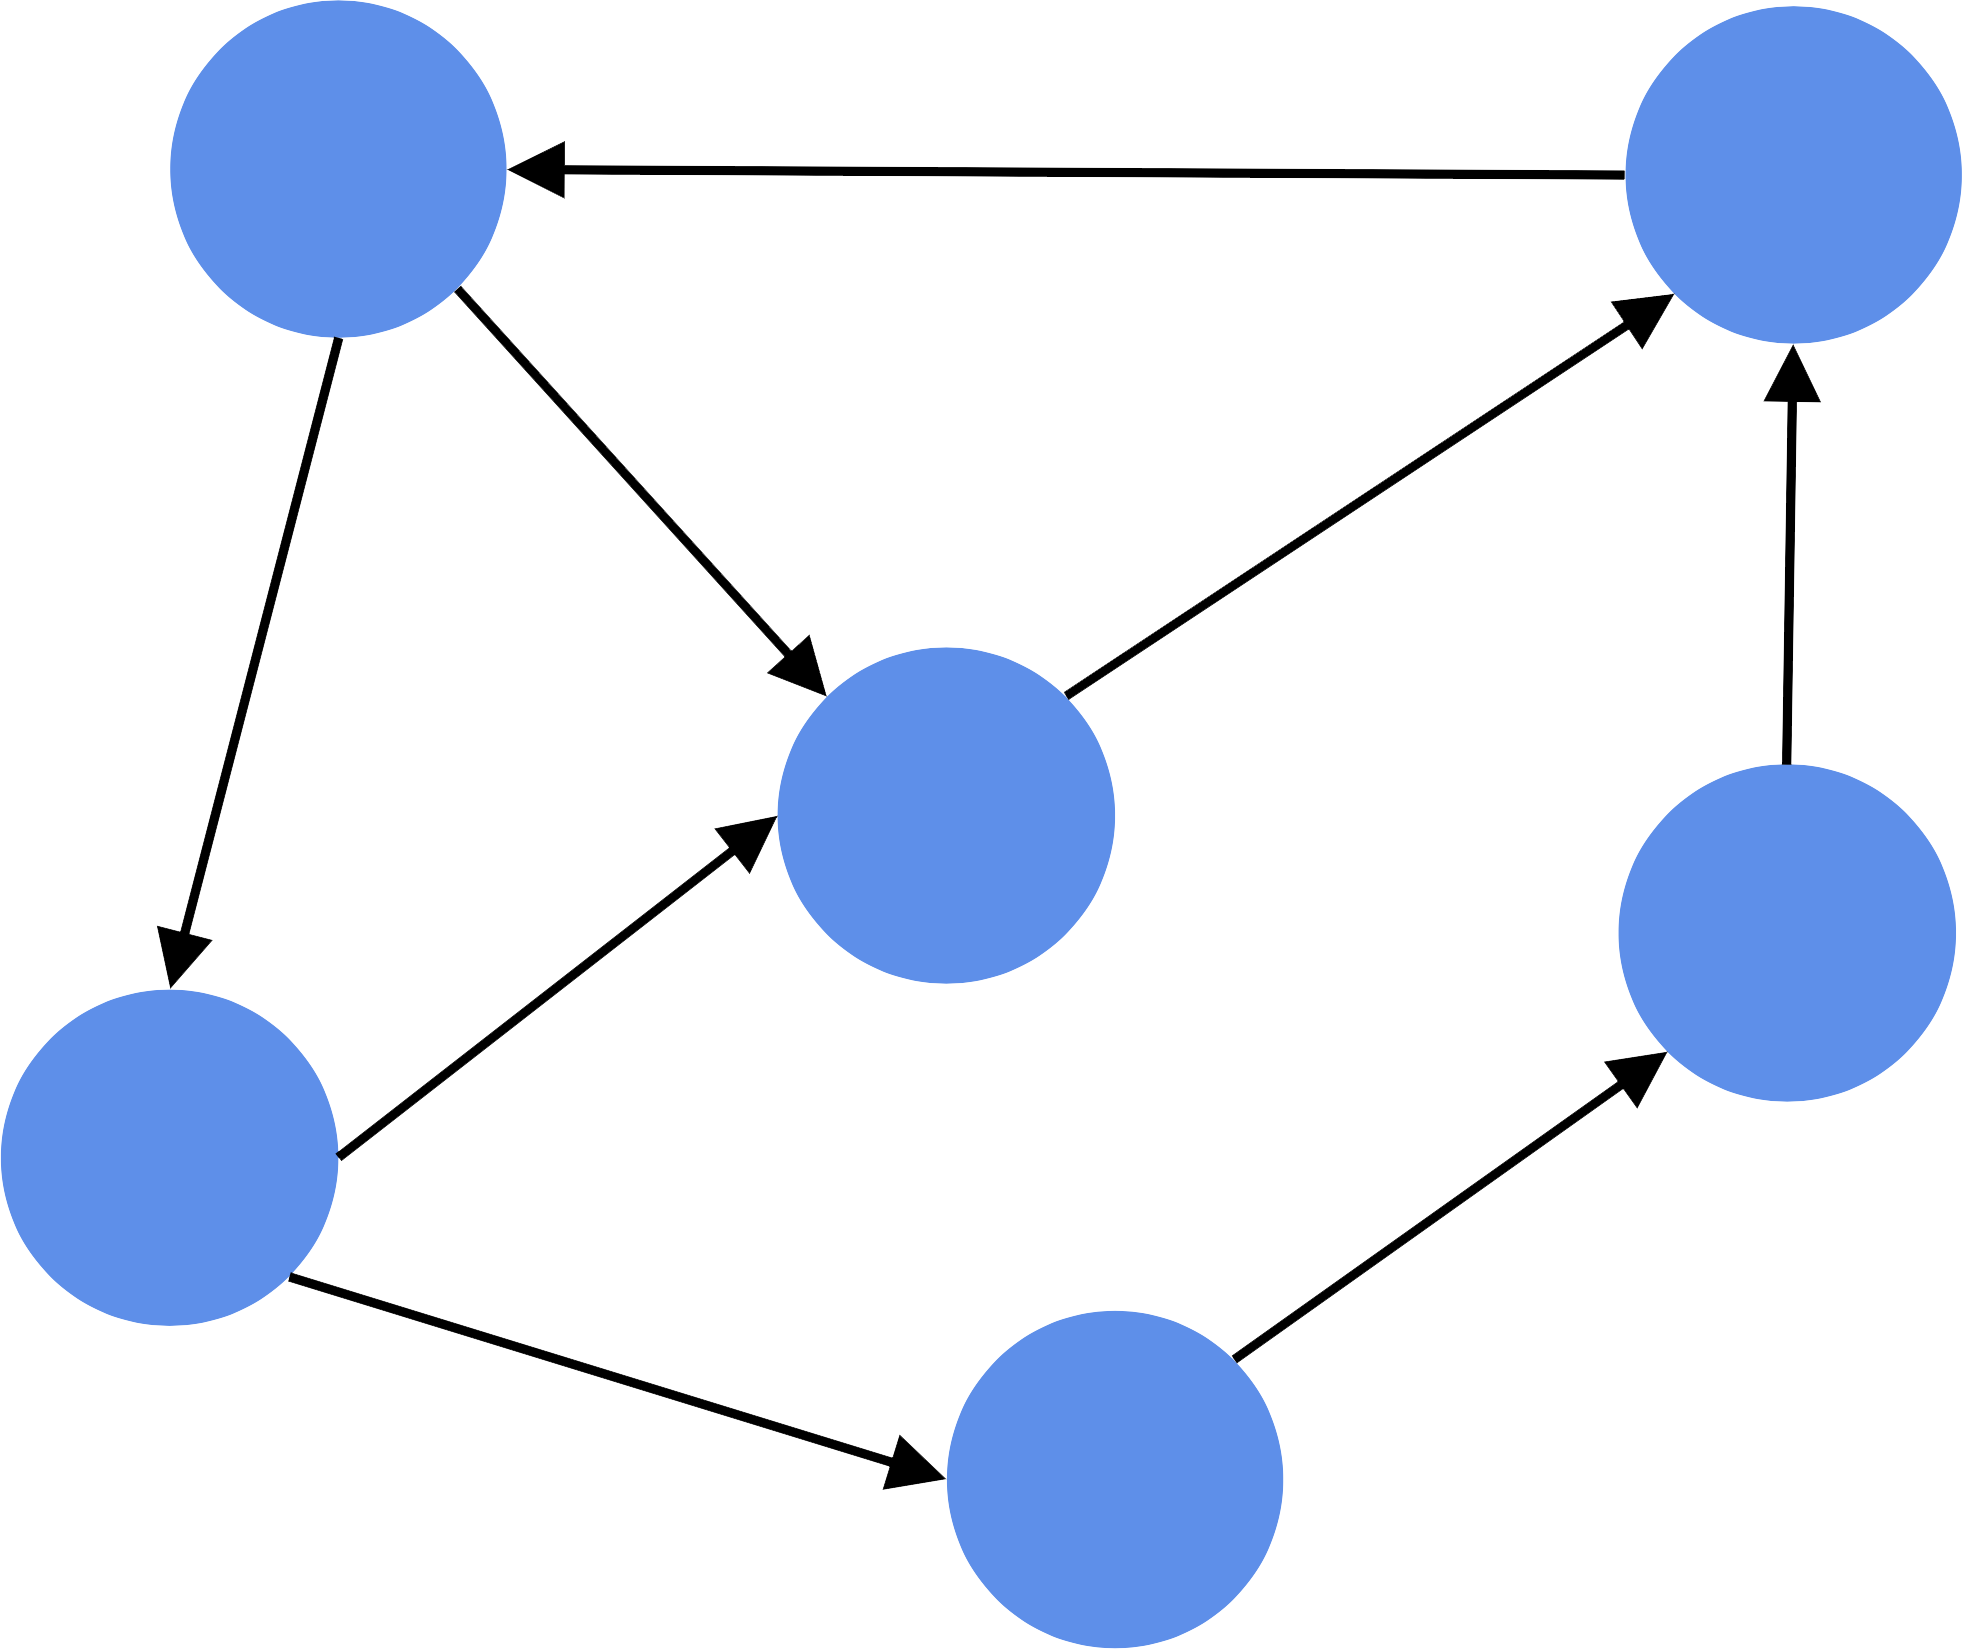
\includegraphics[width=0.2\linewidth]{images/Strongly-Connected.png}
    \qquad
    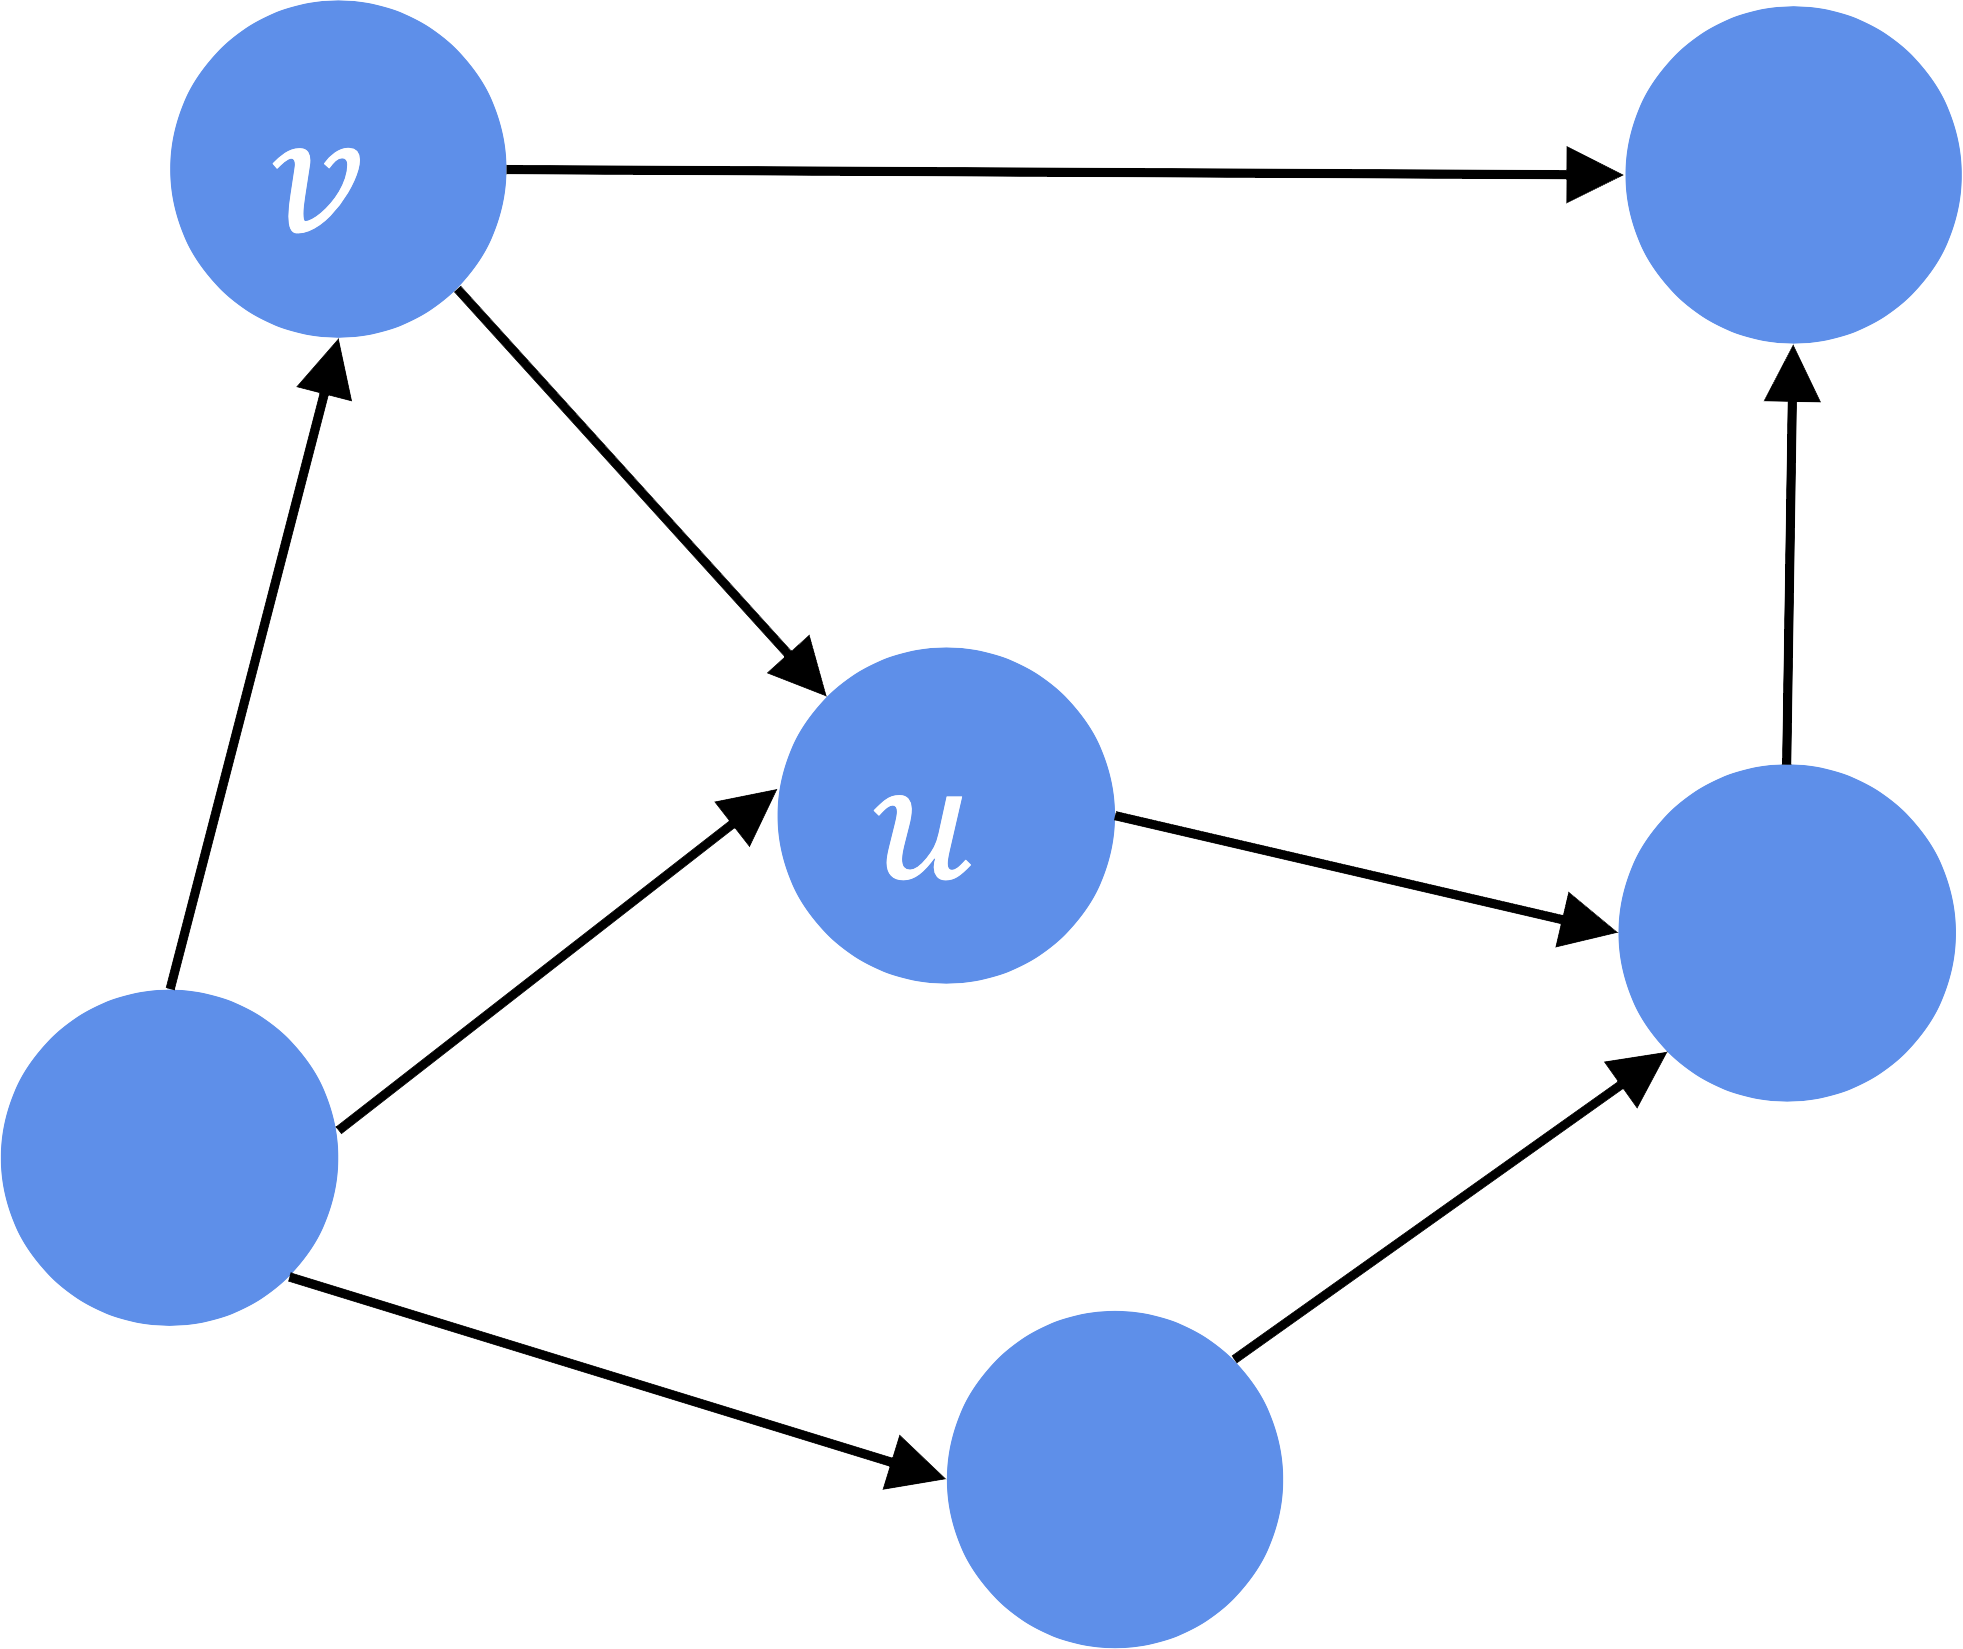
\includegraphics[width=0.2\linewidth]{images/Not-Strongly-Connected.png}
    \caption*{A strongly connected graph (left) and a non-strongly connected graph (right, where $v$ is not reachable from $u$)}
\end{figure}

\listu {
    \item Run \textsc{DFS} on the \bred{transpose} of $G$ (reverse edge direction of all edges in $G$)
    \item \itblue{Reorder} vertices in decreasing order of finish time (in $G.V$ and within each adjacency list)

    Run \textit{DFS} on $G$ using the new ordering of vertices

    \item Each DFS tree is one strongly connected component
}

\section{Minimum Spanning Trees}

\section{Disjoint Sets}